\chapter{Survey}

\section{LTE-A Network Architecture}
{
    The high-level network architecture of LTE is comprised of following three main components:
    \begin{itemize}
        \item The User Equipment (UE).
        \item The Evolved UMTS Terrestrial Radio Access Network (E-UTRAN).
        \item The Evolved Packet Core (EPC).
    \end{itemize}

    \begin{figure}[ht]
        \centering
        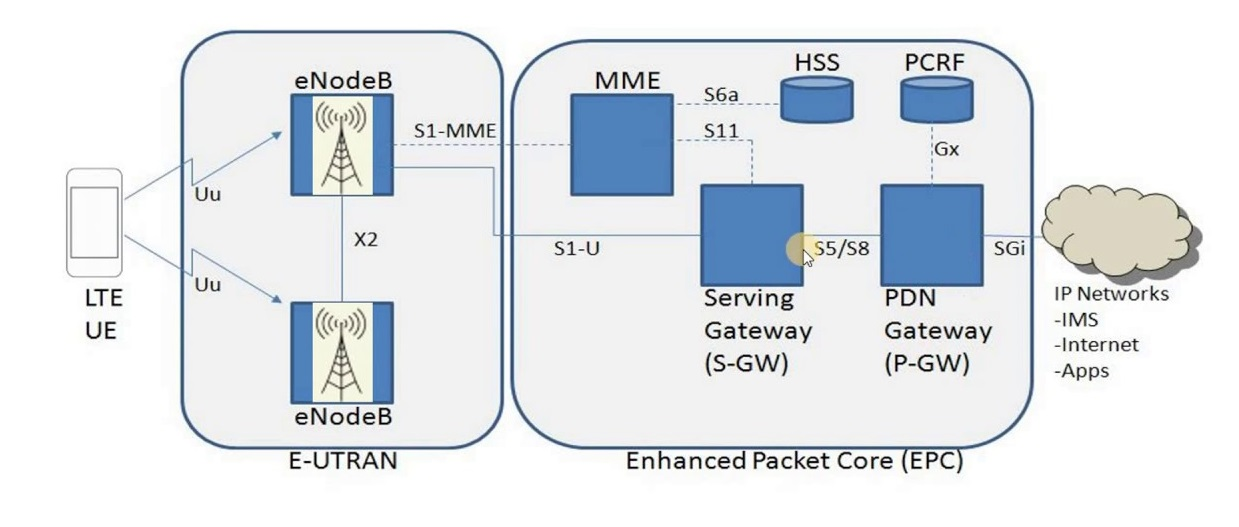
\includegraphics[scale=0.5]{img/LTEA.jpg}
        \caption{LTE-A Network Model for Authentication}
    \end{figure}
}

\subsection{User Equipment (UE)}{
    The internal architecture of the user equipment for LTE is identical 
    to the one used by UMTS and GSM which is actually a Mobile Equipment (ME).
    The mobile equipment comprised of the following important modules:
    \begin{itemize}
        \item \textbf{Mobile Termination (MT) :} This handles all the communication functions.
        \item \textbf{TTerminal Equipment (TE) :} This terminates the data streams.
        \item \textbf{Universal Integrated Circuit Card (UICC) :} This is also known as 
        the SIM card for LTE equipments. It runs an application known as the 
        Universal Subscriber Identity Module (USIM).
    \end{itemize}
    A USIM stores user-specific data very similar to 3G SIM card. This keeps 
    information about the user's phone number, home network identity and security 
    keys etc.
}

\subsection{The E-UTRAN }
{
    The E-UTRAN handles the radio communications between the mobile 
    and the evolved packet core and just has one component, the evolved 
    base stations, called eNodeB or eNB. Each eNB is a base station 
    that controls the mobiles in one or more cells. The base station 
    that is communicating with a mobile is known as its serving eNB.

    \begin{figure}[ht]
        \centering
        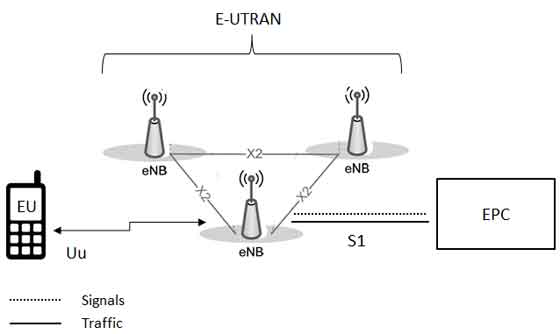
\includegraphics[scale=0.5]{img/ultran.jpg}
        \caption{E-ULTRAN (Access Network)}
    \end{figure}
}

\subsection{The Evolved Packet Core (EPC)}
{
    The EPC represents the Core of an LTE network. It is formed by multiple 
    nodes, the main ones being MME, SGW, PGW and HSS. \\
    It has following functionality:
    \begin{itemize}
        \item Makes the LTE core network function 
        \item Authenticates subscribers
        \item Determines the subscribers’ access to the network
        \item Helps to locate the UE
        \item Essentially aids mobility management
    \end{itemize}
    
    \begin{figure}[h]
        \centering
        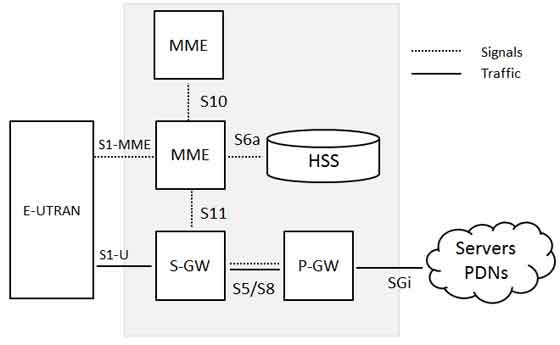
\includegraphics[scale=0.5]{img/epc.jpg}
        \caption{EPC (Core Network)}
    \end{figure}
    
    }

\section{Increasing Network Capacity}{
    In time, as more customers use the mobile network, traffic may build up
    so that there are not enough frequency bands assigned to a cell
    to handle its calls. A number of approaches have been used to cope with this 
    situation, including the following:
    \begin{itemize}
        \item \textbf{Adding new channels:} Typically, when a system is set up
        in a region, not all of the channels are used, and growth and
        expansion can be managed in an orderly fashion by adding
        new channels.
        \item \textbf{Frequency borrowing:}  In the simplest case, frequencies
        are taken from adjacent cells by congested cells. The frequencies can also be assigned to cells dynamically.
        \item \textbf{Cell splitting:} In practice, the distribution of traffic and 
        topographic features is not uniform, and this presents opportunities of 
        capacity increase. Cells in areas of high usage can be split into smaller 
        cells. Generally, the original cells are about 6.5 to 13 km in size. The 
        smaller cells can themselves be split; however, 1.5 km cells are close to 
        the practical minimum size as a general solution. To use a smaller cell, the 
        power level used must be reduced to keep the signal within the cell. Also, 
        as the mobile units move, they pass from cell to cell, which requires 
        transferring of the call from one base transceiver to another. This process 
        is called a handoff. As the cells get smaller, these handoffs become much more 
        frequent.
        \begin{figure}[h]
            \centering
            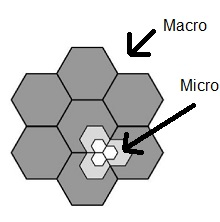
\includegraphics[scale=0.5]{img/split.jpg}
            \caption{Cell Spliting}
        \end{figure}
        \item \textbf{Cell sectoring:} With cell sectoring, a cell is divided into a 
        number of wedgeshaped sectors, each with its own set of channels, typically 
        3 or 6 sectors per cell. Each sector is assigned a separate subset of the 
        cell’s channels, and directional antennas at the base station are used 
        to focus on each sector.
        \begin{figure}[h]
            \centering
            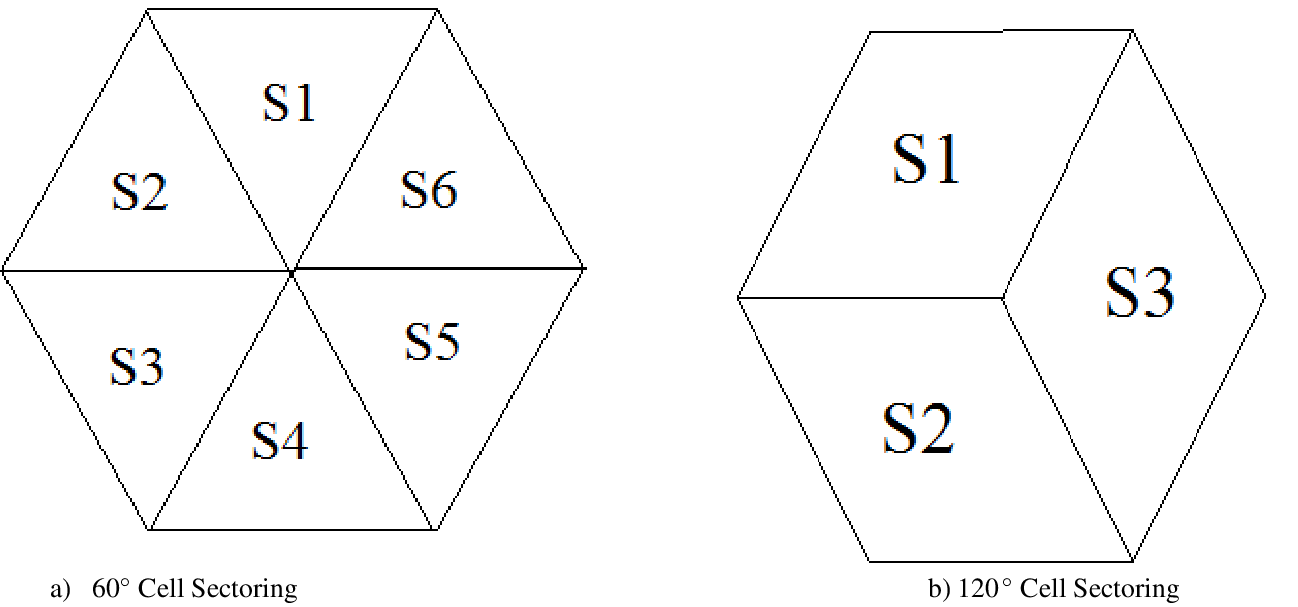
\includegraphics[scale=0.15]{img/sector.png}
            \caption{Cell Sectoring}
        \end{figure}
        \item \textbf{Microcells:} As cells become smaller, antennas move from the 
        tops of tall buildings or hills, to the tops of small buildings or the 
        sides of large buildings, and finally to lamp posts, where they form 
        microcells. Each decrease in cell size is accompanied by a reduction 
        in the radiated power levels from the base stations and the mobile units. 
        Microcells are useful in city streets in congested areas, along highways, 
        and inside large public buildings.
    \end{itemize}
}
    
\section{5G Network Architecture}
{
    \begin{figure}[h]
        \centering
        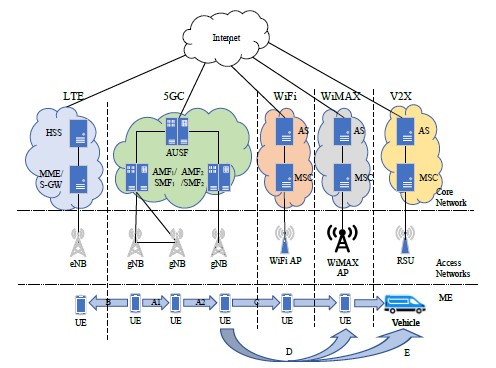
\includegraphics[scale=0.7]{img/5g-arch.jpg}
        \caption{Handover scenarios in 5G networks}
    \end{figure}
    In 5G network, spectrum will come from frequency bands above 24 GHz. Due to high 
    frequency, it will propagate over much shorter distances which is suitable 
    for smaller cells as the interfere between densely deployed cell will be less. This will
    significantly increase the number of base stations. As the earlier network generation
    5G should coexist with previous generation networks.\\ 
    5G network mainly consists of two parts, named Core Network (CN) and Radio Acess 
    Network (RAN) as shown in the above fig. 2.4. 


    \subsection{Core Network}
    {
        CN mainly contains Access and Mobility Management  Function (AMF), 
        User Plane Function (UPF), Session Management Function (SMF), and Authentication 
        Server Function (AUSF). 
        \begin{itemize}
            \item The Access and Mobility Management Function (AMF) acts as a single-entry point for the UE connection.
            \item The User Plane Function (UPF) transports the IP data traffic (user plane) between the User Equipment (UE) and the external networks.
            \item The Authentication Server Function (AUSF) allows the AMF to authenticate the UE and access services of the 5G core.
            \item Other functions like the Session Management Function (SMF), the Policy Control Function (PCF), the Application Function (AF) and the Unified Data Management (UDM) function provide the policy control framework, applying policy decisions and accessing subscription information, to govern the network behavior.
        \end{itemize}
    }


    \subsection{Radio Access Network}{
        In RAN, there are g-Node Base Stations (gNB) which
        communicate with MEs. If a ME wants to connect to the 5G
        CN, AMF would firstly represent AUSF to perform mutual
        authentication with the ME.
    }
    \begin{figure}[h]
        \centering
        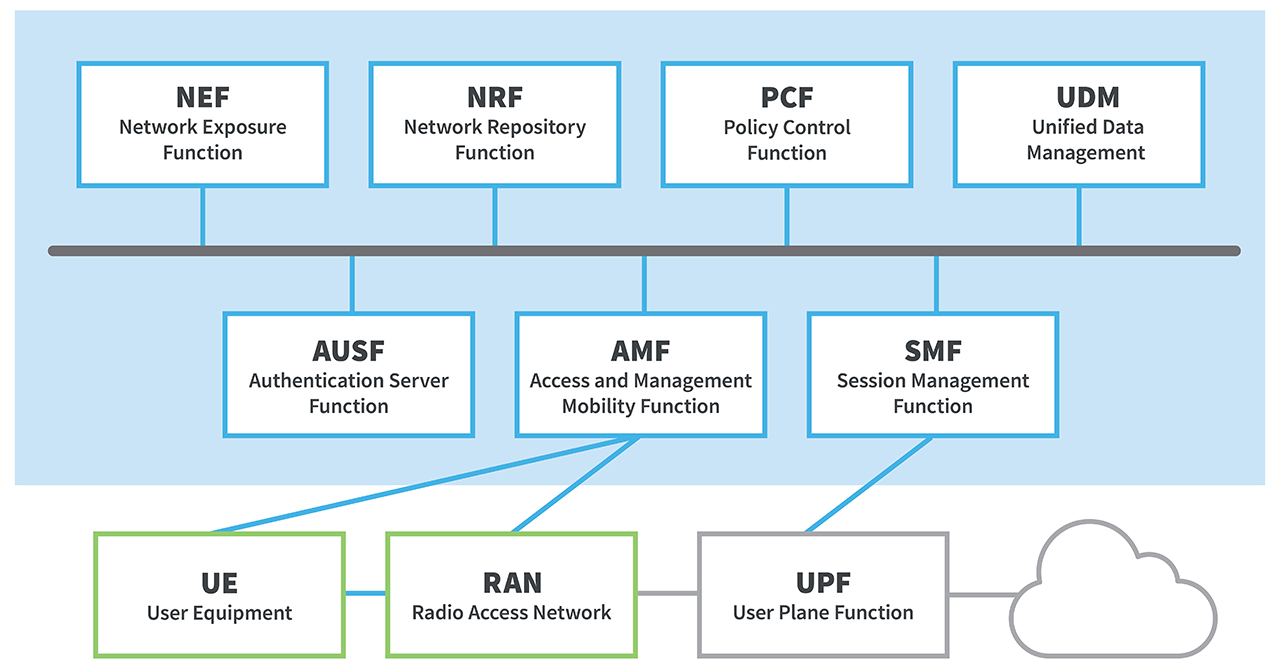
\includegraphics[scale=0.6]{img/5g-rpc.jpg}
        \caption{Key Component of 5G Core Network}
    \end{figure}
}

\section{Threat Model}
{
    
    According to a survey, which have analised 34 types of attacks which are analysed 
    and prevented by authentication and privacy preserving schemes for 4G
    and 5G cellular networks. They have divided these attacks in 4 types as shown in the fig.
    \begin{itemize}
        \item Attacks against privacy
        \item Attacks against integrity
        \item Attacks against availability
        \item Attacks against authentication
    \end{itemize}

    \begin{figure}[h]
        \centering
        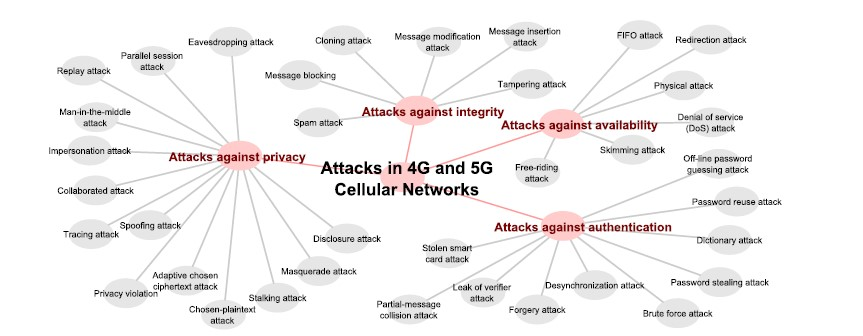
\includegraphics[scale=0.73]{img/attack.jpg}
        \caption{Classification of Attack in 4G/5G Network}
    \end{figure}
    

}
    
\section{Security Requirement}
{
    It describe functional and non-functional requirements that need to be satisfied 
    in order to achieve the security attributes of a network.\\
    It has divided into 6 parts:
    \subsection{Mutual Authentication and Authorization}{
        Authentication is the most important part of the handover security. It is 
        the process of determining whether someone or something is, in fact, who 
        or what it says it is.An ME should be successfully authenticated by both 
        its source network and its target network whenever a handover occurs. On 
        the other hand, the ME must confirm the validity of the target network
        before accessing it. After the success of mutual authentication,
        subscribed services should be negotiated and authorized for the
        ME. The requirements on mutual authentication and authorization
        mainly prevent the handover in 5G networks from attacks
        against authentication, e.g., impersonation attacks, spoofing
        attacks, and MitM attacks.
    }

    \subsection{Confidentiality}{
        Confidentiality is the ability not to disclose information to unauthorized 
        persons, programs, or processes. It relates to information security 
        because it requires control over access to protected information. 
        Confidentiality requires measures to ensure that only authorized 
        persons have access to information, and while unauthorized persons 
        are denied access to them. Simply put, confidentiality means that 
        something is secret and should not be passed on to unintentional persons 
        or organizations. If confidentiality is compromised, this can lead to 
        loss of privacy and disclosure of confidential information to the public 
        or other persons. 
    }
    \subsection{Integrity}{

        Integrity means that protection against improper modification and 
        destruction of information, ensuring that information cannot be 
        changed undetected, and ensuring the integrity of the information. 
        This means that a cyber threat or vulnerability to cyber-attack can 
        be measured by compromising one or more of its principles. Integrity 
        is based on encryption and hashing to ensure the best possible 
        protection against cyber attacks and cyber threats such as cyber espionage.\\

        This is a basic security requirement for the 5G networks, naturally
        also for handover. Correspondingly, ME and the network
        should agree on a session key after the handover in order to
        achieve confidentiality and integrity in each communication
        session against both passive attacks, such as eavesdropping,
        and active attacks, such as message blocking attacks, message
        modification attacks, and tampering attacks.
    }
    \subsection{Availability}{
        Availability means that the network is
        available for legal users in any situation even under common
        attacks. The services should be robust anytime and anywhere
        even under DoS or DDoS attacks. Since 5G is an open
        environment, an adversary can attack ME or BS from different
        networks by raising various kinds of attacks.
    }
    \subsection{Resistent to active and passive attacks}{
        \textbf{Active attack: } An Active attack attempts to alter system resources or affect their operations. Active attacks involve some modification of the data stream or the creation of false statements. \\[0.6\baselineskip]
        \textbf{Passive attack: } A Passive attack attempts to learn or make use of information from the system but does not affect system resources. Passive Attacks are in the nature of eavesdropping on or monitoring transmission. The goal of the opponent is to obtain information that is being transmitted.

    }
    \subsection{Session Key Secrecy}{
        A session key is an encryption and decryption key that is randomly 
        generated to ensure the security of a communications session between 
        a user and another computer or between two computers.\\
        Securing session is also very important. It contains 3 parts:
        \subsubsection{Forward/Backward Secrecy}{
            \begin{itemize}
                \item \textbf{Forward Secrecy: } It is a feature
                that for an entity with knowledge of session key \(K_m\) between
                the entity with a second entity, it is infeasible to predict
                any future \(K_{m+n}\) (n$>$0) used between a third entity and the
                second entity. Forward secrecy protects future communications
                from the threat of current keys leakage. In the context of
                handover, forward secrecy refers to the property that, for a
                gNB with knowledge of a \(K_{gNB}\), shared with a UE, it is
                computationally infeasible to predict any future \(K_{gNB}\) that
                will be used between the same UE and another gNB.

                \item \textbf{Backward Secrecy: }{
                    Contrary to FWS, Backward Secrecy
                    (BWS) is a feature that for an entity with knowledge of
                    session key \(K_n\), it is infeasible to predict any previous \(K_{n-m}\)
                    (n$>$m$>$0) from which \(K_n\) is derived. Backward secrecy
                    protects previous communications from the threat of current
                    keys leakage. In the context of handover, backward secrecy
                    refers to the property that, for a gNB with knowledge of a
                    KgNB, shared with a UE, it is computationally infeasible to
                    predict any previous \(K_{gNB}\) that has been used between the
                    same UE and a previous gNB.
                }
            \end{itemize}
        }

        \subsubsection{Key Escrow Freshness}{
            Key escrow is a method of storing important cryptographic keys. Each key stored in an escrow system is tied to the original user and subsequently encrypted for security purposes. Much like a valet or coat check, each key is stored in relation to the user that leverages it, and then returned once queried. By using key escrow, organizations can ensure that in the case of catastrophe, be it a security breach, lost or forgotten keys, natural disaster, or otherwise, their critical keys are safe.
        }
        \subsubsection{Ephemeral Secret Leakage}{
            If ephemeral secrets are compromised, an adversary can reveal the private keys of clients and the session key would turn out to be known from the eavesdropped messages. This phenomenon is called Ephemeral Secret Leakage (ESL) attacks.
        }
        
    }
    \subsection{Privacy}{
        \subsubsection{Conditional Privacy}{
            Although it is quite significant
            to preserve user privacy, some sensitive information is requested
            to be provided in order to offer some services in
            certain situations. For example, when a user falls into a
            dangerous situation and needs help, his/her location should
            be conditionally available to ambulancemen. Thus, conditional
            privacy should be offered in the 5G handover.
        }
        \subsubsection{Non Traceability}{
            To distribute pseudonyms to the
            mobile user is a good way to achieve anonymity, but the
            adversary is able to trace users by linking a number of
            fixed pseudonyms between different sessions. Therefore, it is
            necessary to ensure non-traceability in handover.
        }
        \subsubsection{Anonymity}{
            In many handover
            scenarios in 5G networks, user identity privacy preservation
            is a significant requirement. Mobile users prefer to enjoy
            seamless mobile network services without using their real
            identities and exposing locations or other personally sensitive
            information. The real identity of an ME must be hidden from
            visiting networks or other MEs, and no attacker can link
            specific conversations to the real identity so that the user’s
            privacy can be well protected from various attacks against
            privacy.
        }
    }

}

\section{Possible Solution of Security Requirement}{
    \subsection{Mutual Authentication}{
        Mutual Authentication is a security process in which entities authenticate each other before actual communication occurs.
    }
    \subsection{Proper Key agreement}{
        Key exchange protocols enable two or more parties to establish a shared encryption key that they can use to encrypt or sign data that they plan to exchange. Key exchange protocols typically employ cryptography to achieve this goal. Different cryptographic techniques can be used to achieve this goal.\\

        In order for two parties to communicate confidentially, they must first exchange the secret key that will be used to encrypt and decrypt messages. This initial exchange of the encryption key is called the key exchange.\\

        A proper key exchange protocol is to be designed to establish confidentiality 
        without letting unauthorized party to intercept, infer or otherwise obtain the key. 

    }
    \subsection{Dynamic Key}{
        In traditional cryptosystems a specific cipher is chosen thus security of the system relies on the frequency of key changes and the key agreement scheme. Dynamic Encryption enhance such a system by defining a set of ciphers such that not only the key but also the cipher changes on every new data transaction.
    }
    \subsection{Desynchronization Resistant}{
        A connection should be maintain even after any type attack 
    }
    \subsection{Dynamic Pseudonym}{
        Identity protection is considered to be important for authentication and key agreement protocol design in single-server and multi-server architectures.
        For that Dynamic Pseudonym should be used.
    }
    \subsection{Short-term and Long-term Key}{
        If Alice and Bob are going to speak securely, they don't need to keep the shared secret key around for a long time. They only need it for as long as they're speaking. And they don't want someone who records their conversation to be able to learn what they said. If they agree on a temporary key, one that lasts only as long as their conversation, that is a session key.

        A session key is one that is not intentionally stored, and is not re-creatable. Session keys are used only for communications protocols, never for storage purposes. In computer protocols like SSL, the session key is generated randomly, exchanged securely with the other computer (using a key exchange protocol like DH), and remains in each computer's memory only for the duration it is needed (a session.) When the session is ended, both sides wipe their copies of the key from memory.*

        A long-term key is one that is deliberately stored somewhere, either on a computer disk, flash memory, or even printed on paper. The key is intended to be used at multiple points in time, such as "I will use this key to encrypt this secret file today, and use it again to decrypt my secret next week." A long term key can be used for any purpose, including stored information as well as transient communications.
    }
}